\documentclass[11pt]{article}
\usepackage{graphicx} % Required for inserting images
\usepackage{babel}[polish]
%\usepackage{polski}
\usepackage{float}
\usepackage{adjustbox}
\usepackage{subfig}
\usepackage{booktabs}
\usepackage{siunitx}
\usepackage[a4paper,top=2cm,bottom=2cm,left=3cm,right=3cm,marginparwidth=1.75cm]{geometry}
\usepackage{tikz}
\usepackage{pgfplots}
\usepackage{pgfplotstable}
\usepackage{amsmath}
\usepackage{tabularx}
\usepackage{array}
\newcolumntype{Y}{>{\centering\arraybackslash}X}
\usepackage{xcolor,colortbl}
\usepackage{titling}

\pgfplotsset{compat=newest}
\usepgfplotslibrary{external}
\tikzexternalize[prefix=tikz/]

\title{ELA2 - Projekt}
\author{Piotr Pokornowski 325061}
\date{\today}

%\pgfplotstableread[col sep=semicolon]{figures/digital/output.csv}\digital

\pgfplotsset{select coords between index/.style 2 args={
            x filter/.code={
                    \ifnum\coordindex<#1\def\pgfmathresult{}\fi
                    \ifnum\coordindex>#2\def\pgfmathresult{}\fi
                }
        }}


        \pgfplotsset{
    tick scale binop/.code args={#1:#2}{%
        \pgfkeysalso{/pgfplots/tick label style={/pgf/number format/fixed, /pgf/number format/fixed zerofill=true}}%
        \pgfmathparse{#2*pow(10,#1)}%
    },
    xtick scale label/.style={
        scaled x ticks=manual:#1,
        xtick scale binop=#1,
        xticklabel={$\pgfmathprintnumber{\tick}$}
    },
    ytick scale label/.style={
        scaled y ticks=manual:#1,
        ytick scale binop=#1,
        yticklabel={$\pgfmathprintnumber{\tick}$ mA}
    }
}

\begin{document}

\begin{titlingpage}
    \maketitle
\end{titlingpage}

\section{Sekcja cyfrowa}
\subsection{Opis układu}
Zaprojektowana przetwornica obniża napięcie z \SI{10}{\V} do \SI{5}{\V} i działa dla prądu maksymalnego \SI{5}{\A}. Jej zadaniem jest zasilanie cyfrowej sekcji układu, z tego powodu minimalizacja tętnień była celem drugorzędnym, a priorytetem stało się uzyskanie jak największej sprawności \textemdash \ dla maksymalnego obciążenia prądem \SI{5}{\A} udało się uzyskać sprawność na poziomie $\sim \SI{94.3}{\percent}$.

\begin{figure}[H]
    \centering
    \captionsetup{justification=centering}
    \begin{adjustbox}{width=1.1\textwidth,center}
        \subfloat[Schemat układu]{
            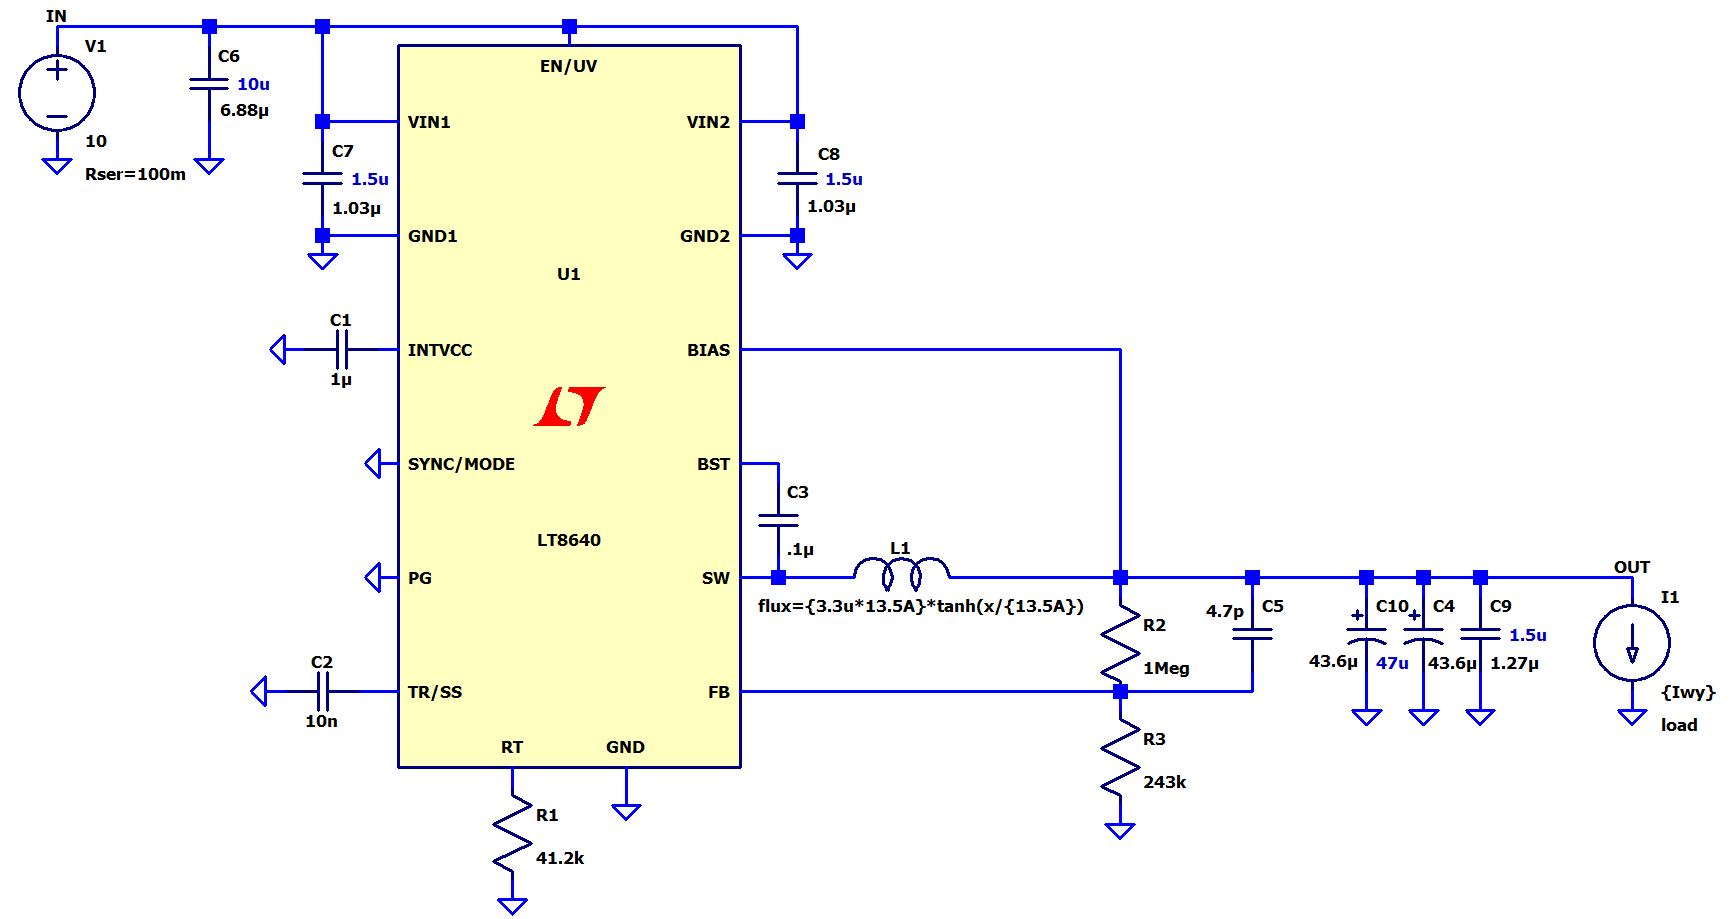
\includegraphics[width=\textwidth]{./figures/digital/digital.png}
            \label{fig:subfig1}
        }
        \qquad
        \subfloat[Przebiegi czasowe prądu i napięcia na wyjściu układu \\ przy maksymalnym obciążeniu]{
            \begin{tikzpicture}
                \pgfplotsset{
                    scale only axis,
                    scaled x ticks=base 10:3,
                    xmin=0, xmax=0.008
                }

                \begin{axis}[
                        grid=both,
                        axis y line*=left,
                        ymin=-1, ymax=6,
                        xlabel={Czas $t$ [s]},
                        ylabel={Napięcie wyjściowe $V_{\text{OUT}}$ [V]},
                    ]
                    \addplot[green, thick] table {./figures/digital/vout/segment_1.csv};\label{vout}
                    \addplot[green, thick] table {./figures/digital/vout/segment_2.csv};
                    \label{plot:vout}
                \end{axis}

                \begin{axis}[
                        axis y line*=right,
                        axis x line=none,
                        ymin=-1,
                        ymax=6,
                        ytick pos=right,
                        yticklabel pos=right,
                        ytick distance=1,
                        ylabel={Prąd wyjściowy $I_{\text{OUT}}$ [A]},
                        legend style={at={(0.95,0.05)},anchor=south east},
                    ]
                    \addlegendimage{/pgfplots/refstyle=vout}
                    \addlegendentry{$V_{OUT}$}
                    \addplot[red, thick] table {./figures/digital/iout/segment_1.csv};\label{iout}
                    \addplot[red, thick] table {./figures/digital/iout/segment_2.csv};

                    \addlegendimage{/pgfplots/refstyle=iout}
                    \addlegendentry{$I_{OUT}$}
                    \label{plot:current}
                \end{axis}
            \end{tikzpicture}

            \label{fig:subfig2}
        }
    \end{adjustbox}
\end{figure}

\subsection{Wybór elementów}
\subsubsection{Wybór LT8640}
Wykorzystany układ LT8640 został wybrany, ponieważ spełniał wymagania projektowe oraz był dostępny w dużych ilościach wśród dostawców. Dodatkowo, Analog Devices sugeruje go jako jeden z układów do wykorzystania przy nowych projektach.

\subsubsection{Dobór cewki}
Cewka została dobrana zgodnie ze wzorem
\[
    L = \frac{V_{OUT} + V_{SW(BOT)}}{f_{SW}} \approx \SI{3.6}{\micro\henry}
\]
dostępnym w nocie katalogowej. W układzie znalazła się więc najbliższa z szeregu cewka o wartości \SI{3.3}{\micro\henry}. Podobna cewka o takiej samej wartości jest używana w przykładowym układzie producenta.

\subsubsection{Dobór kondensatorów}
Kondensatory zostały dobrane zgodnie z zaleceniami producenta układu, jednocześnie biorąc pod uwagę spadek pojemności. Wszystkie użyte kondensatory to kondensatory MLCC, z wyjątkiem dwóch dużych kondensatorów wyjściowych. Zamiast MLCC użyte są tam aluminiowe kondensatory elektrolityczne, co pozwoliło na znaczną redukcję kosztów przy zachowaniu dobrych parametrów. Wykorzystanie w tym miejscu trudno dostępnych kondensatorów ceramicznych o pojemności \SI{47}{\micro\farad} byłoby nieopłacalne, gdyż kosztowały one więcej niż cała reszta elementów w układzie.

\subsection{Wyniki symulacji}
\begin{table}[H]
    \centering
    \caption{Porównanie wyników symulacji w zależności od obciążenia}
    \label{tab:efficiency_ripple}
    \begin{tabular}{ccccc}
        \toprule
        \textbf{Prąd obciążenia [mA]} & \textbf{Sprawność [\%]} & $\mathbf{\Delta{V_{IN}} \ [mV]}$ & $\mathbf{\Delta{V_{OUT}} \ [mV]}$ & $\mathbf{V_{AVG} \ [V]}$ \\
        \midrule
        0.0                           & 0.00                    & 0.00                             & 0.68                              & 5.03                     \\
        0.5                           & 97.76                   & 147.75                           & 69.52                             & 4.96                     \\
        1.0                           & 97.99                   & 234.75                           & 70.82                             & 4.96                     \\
        1.5                           & 97.70                   & 316.64                           & 72.18                             & 4.96                     \\
        2.0                           & 97.28                   & 402.93                           & 70.74                             & 4.95                     \\
        2.5                           & 96.82                   & 485.24                           & 71.01                             & 4.95                     \\
        3.0                           & 96.33                   & 565.54                           & 70.95                             & 4.95                     \\
        3.5                           & 95.92                   & 649.69                           & 71.78                             & 4.95                     \\
        4.0                           & 95.31                   & 730.42                           & 73.02                             & 4.95                     \\
        4.5                           & 94.80                   & 813.73                           & 74.20                             & 4.95                     \\
        5.0                           & 94.28                   & 899.40                           & 75.92                             & 4.95                     \\
        \bottomrule
    \end{tabular}
\end{table}

\subsection{Wnioski}
Wykorzystanie przetwornicy impulsowej pozwoliło na uzyskanie bardzo dużej sprawności, co byłoby niemożliwe w przypadku stabilizatora liniowego. Wadą takiego rozwiązania jest jednak większe tętnienie napięcia wyjściowego, co w przypadku zasilania cyfrowego układu nie jest problemem. Kolejną zaletą jest również stabilność napięcia wyjściowego przy zmianach obciążenia, co byłoby niemożliwe gdy do obniżenia napięcia wykorzystany byłby np. prosty dzielnik napięciowy.

% ----------------------------------------------

\section{Sekcja analogowa I}
\subsection{Opis układu}
Zaprojektowany układ obniża napięcie z \SI{10}{\V} do \SI{5}{\V} i działa dla prądu maksymalnego \SI{250}{\milli\A}. Jego zadaniem jest zasilanie analogowej sekcji układu, która powinna mieć jak najmniejsze tętnienia. Z tego powodu ten układ został wykonany z użyciem wyłącznie stabilizatora, co powinno zapewnić (przynajmniej w teorii) zerowe tętnienia.

\begin{figure}[H]
    \centering
    \captionsetup{justification=centering}
    \begin{adjustbox}{width=1.1\textwidth,center}
        \subfloat[Schemat układu]{
            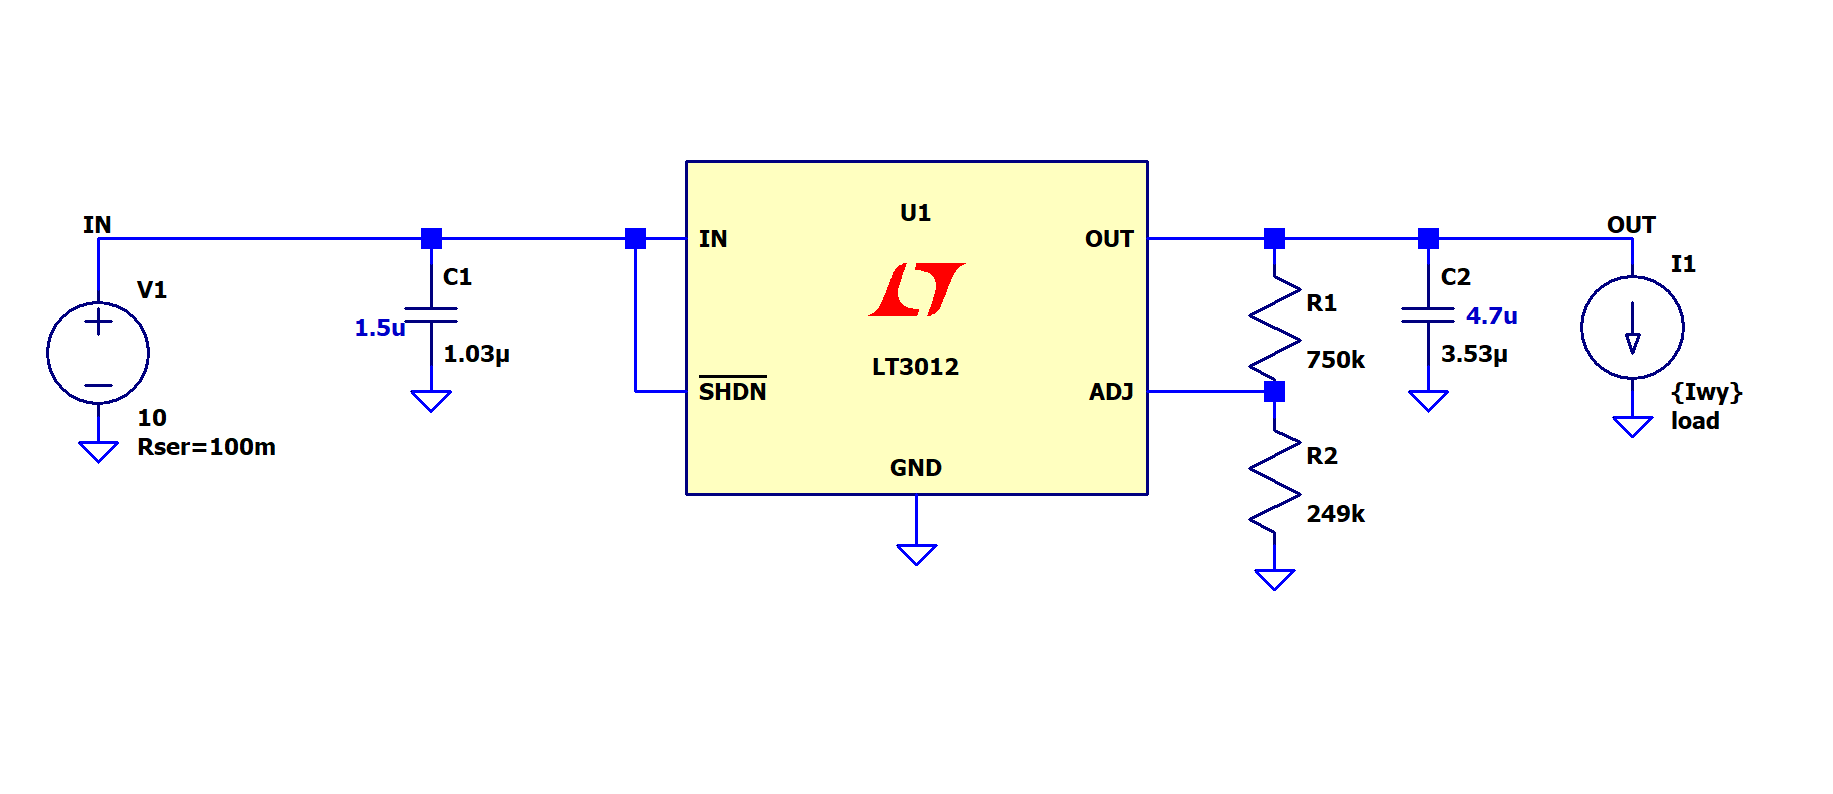
\includegraphics[width=\textwidth]{./figures/analog_1/schematic.png}
            \label{fig:subfig1}
        }
        \qquad
        \subfloat[Przebiegi czasowe prądu i napięcia na wyjściu układu \\ przy maksymalnym obciążeniu]{
            \begin{tikzpicture}
                \pgfplotsset{
                    scale only axis,
                    scaled x ticks=base 10:3,
                    xmin=0, xmax=0.008
                }

                \begin{axis}[
                        grid=both,
                        axis y line*=left,
                        ymin=-1, ymax=6,
                        xlabel={Czas $t$ [s]},
                        ylabel={Napięcie wyjściowe $V_{\text{OUT}}$ [V]},
                    ]
                    \addplot[green, thick] table {./figures/analog_1/vout/vout.txt};\label{vout}
                    \label{plot:vout}
                \end{axis}

                \begin{axis}[
                        axis y line*=right,
                        axis x line=none,
                        ymin=-0.050,
                        ymax=.300,
                        ytick pos=right,
                        yticklabel pos=right,
                        ytick = {-0.05, 0, 0.05, 0.1, 0.15, 0.2, 0.25, 0.3},
                        yticklabels = {-50, 0, 50, 100, 150, 200, 250, 300},
                        ylabel={Prąd wyjściowy $I_{\text{OUT}}$ [mA]},
                        legend style={at={(0.95,0.05)},anchor=south east},
                    ]
                    \addlegendimage{/pgfplots/refstyle=vout}
                    \addlegendentry{$V_{OUT}$}
                    \addplot[red, thick] table {./figures/analog_1/iout/iout.txt};\label{iout}

                    \addlegendimage{/pgfplots/refstyle=iout}
                    \addlegendentry{$I_{OUT}$}
                    \label{plot:current}
                \end{axis}
            \end{tikzpicture}
            \label{fig:subfig2}
        }
    \end{adjustbox}
\end{figure}

\subsection{Wybór elementów}
\subsubsection{Wybór stabilizatora}
W układzie został wykorzystany stabilizator LT3012, ponieważ jego parametry spełniają wymagania projektowe, a producent poleca go do wykorzystania w nowych projektach.

\subsubsection{Dobór kondensatorów}
Kondensatory zostały dobrane zgodnie z zaleceniami producenta układu, jednocześnie biorąc pod uwagę spadek pojemności. Wszystkie użyte kondensatory to kondensatory MLCC. Dodatkową kwestią przy ich wyborze, był fakt, że są one już wykorzystywane w sekcji cyfrowej, co pozwoliło na zmniejszenie kosztów.
\subsection{Wyniki symulacji}
\begin{table}[H]
    \centering
    \caption{Porównanie wyników symulacji w zależności od obciążenia}
    \label{tab:efficiency_ripple}
    \begin{tabular}{ccccc}
        \toprule
        \textbf{Prąd obciążenia [mA]} & \textbf{Sprawność [\%]} & $\mathbf{\Delta{V_{IN}} \ [mV]}$ & $\mathbf{\Delta{V_{OUT}} \ [mV]}$ & $\mathbf{V_{AVG} \ [V]}$ \\
        \midrule
        0.0                           & 0                       & 0.0                              & 2.82                              & 5.07                     \\
        25.0                          & 48.38                   & 0.0                              & 0.14                              & 5.01                     \\
        50.0                          & 48.45                   & 0.0                              & 0.14                              & 5.01                     \\
        75.0                          & 48.48                   & 0.0                              & 0.14                              & 5.01                     \\
        100.0                         & 48.49                   & 0.0                              & 0.14                              & 5.01                     \\
        125.0                         & 48.50                   & 0.0                              & 0.14                              & 5.01                     \\
        150.0                         & 48.50                   & 0.0                              & 0.14                              & 5.01                     \\
        175.0                         & 48.51                   & 0.0                              & 0.14                              & 5.01                     \\
        200.0                         & 48.51                   & 0.0                              & 0.14                              & 5.00                     \\
        225.0                         & 48.52                   & 0.0                              & 0.14                              & 5.00                     \\
        250.0                         & 48.52                   & 0.0                              & 0.14                              & 5.00                     \\
        \bottomrule
    \end{tabular}
\end{table}

% ----------------------------------------------

\section{Sekcja analogowa II}
\subsection{Opis układu}
Zaprojektowana przetwornica podnosi napięcie z \SI{10}{\V} do \SI{12}{\V} i działa dla prądu maksymalnego \SI{100}{\milli\A}. Jej zadaniem jest zasilanie analogowej sekcji układu, która powinna mieć jak najmniejsze tętnienia. Układ wykorzystuje przetwornicę LT8362.

\begin{figure}[H]
    \centering
    \captionsetup{justification=centering}
    \begin{adjustbox}{width=1.2\textwidth,center}
        \subfloat[Schemat układu]{
            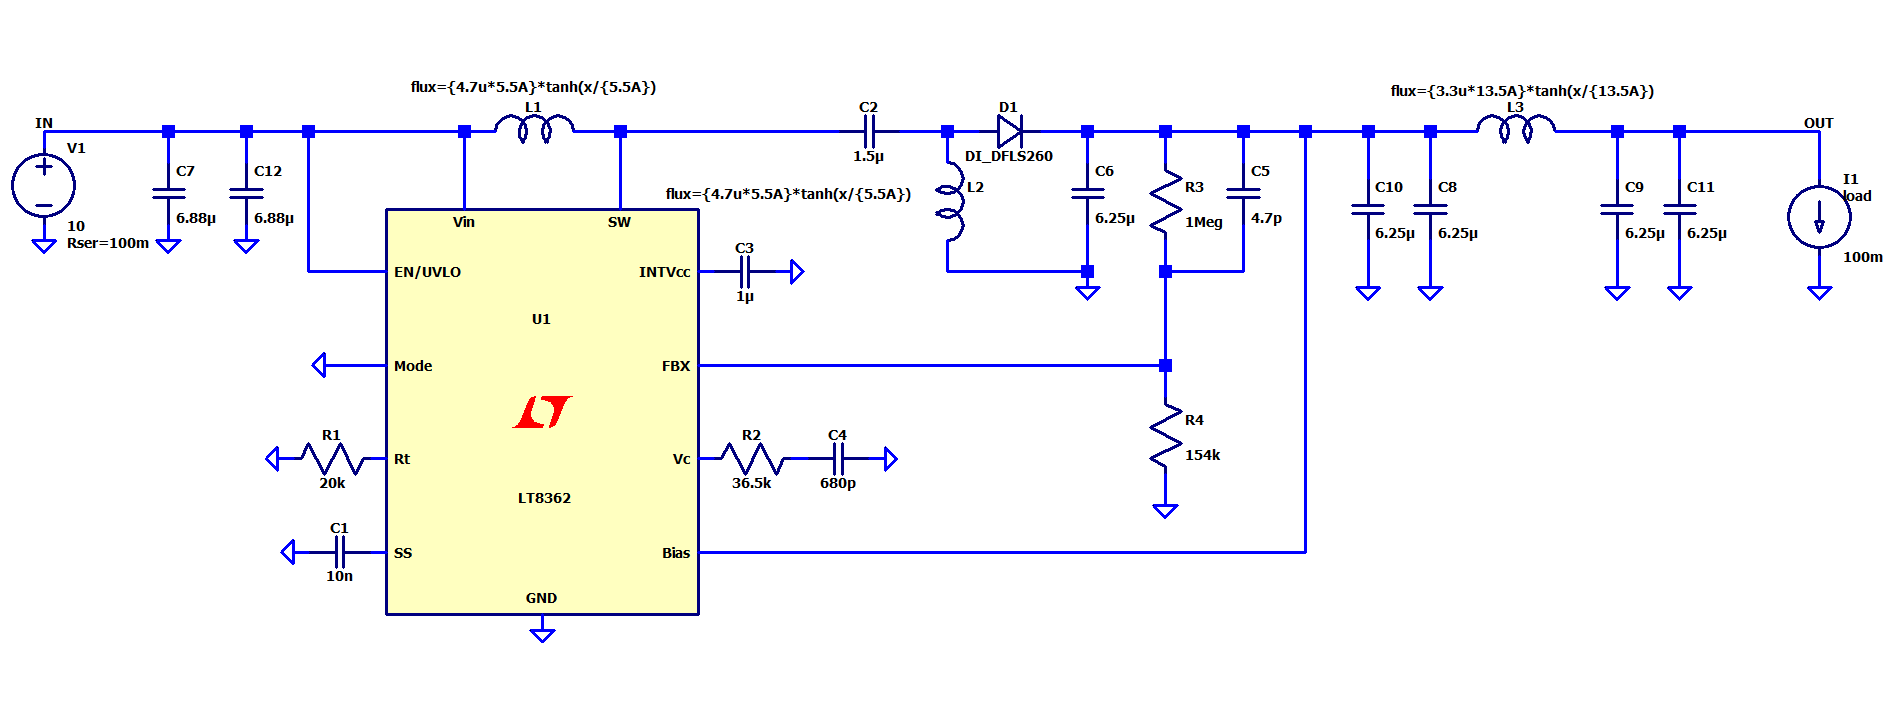
\includegraphics[width=\textwidth]{./figures/analog_2/schematic.png}
            \label{fig:subfig1}
        }
        \qquad
        \subfloat[Przebiegi czasowe prądu i napięcia na wyjściu układu \\ przy maksymalnym obciążeniu]{
            \begin{tikzpicture}
                \pgfplotsset{
                    scale only axis,
                    scaled x ticks=base 10:3,
                    xmin=0, xmax=0.005
                }

                \begin{axis}[
                        grid=both,
                        axis y line*=left,
                        ymin=-1, ymax=13,
                        xlabel={Czas $t$ [s]},
                        ylabel={Napięcie wyjściowe $V_{\text{OUT}}$ [V]},
                    ]
                    \addplot[green, thick] table {./figures/analog_2/vout/segment_1.csv};\label{vout}
                    \addplot[green, thick] table {./figures/analog_2/vout/segment_2.csv};
                    \label{plot:vout}
                \end{axis}

                \begin{axis}[
                        axis y line*=right,
                        axis x line=none,
                        ymin=-0.01,
                        ymax=0.13,
                        ytick pos=right,
                        yticklabel pos=right,
                        ytick = {0, 0.02, 0.04, 0.06, 0.08, 0.1, 0.12},
                        yticklabels = {0, 20, 40, 60, 80, 100, 120},
                        ylabel={Prąd wyjściowy $I_{\text{OUT}}$ [mA]},
                        legend style={at={(0.95,0.05)},anchor=south east},
                    ]
                    \addlegendimage{/pgfplots/refstyle=vout}
                    \addlegendentry{$V_{OUT}$}
                    \addplot[red, thick] table {./figures/analog_2/iout/segment_1.csv};\label{iout}
                    \addplot[red, thick] table {./figures/analog_2/iout/segment_2.csv};

                    \addlegendimage{/pgfplots/refstyle=iout}
                    \addlegendentry{$I_{OUT}$}
                    \label{plot:current}
                \end{axis}
            \end{tikzpicture}

            \label{fig:subfig2}
        }
    \end{adjustbox}
\end{figure}

\subsection{Wybór elementów}
\subsubsection{Wybór LT8362}
Przetwornica obniżająca została wykonana w topologii SEPIC, ponieważ charakteryzują sie one mniejszymi tętnieniami napięcia wyjściowego niż klasyczne przetwornice typu boost. Układ LT8362 został wybrany, ponieważ spełniał wymagania projektowe oraz był dostępny w dużych ilościach wśród dostawców. Dodatkowo, Analog Devices sugeruje go jako jeden z układów do wykorzystania przy nowych projektach.

\subsubsection{Dobór cewki}
Cewka została dobrana zgodnie ze wzorami dostępnym w nocie katalogowej, jednocześnie sugerując się przykładowym układem producenta. W układzie znalazła się cewka o wartości \SI{4.7}{\micro\henry}.

\subsubsection{Dobór kondensatorów}
Kondensatory zostały dobrane zgodnie z zaleceniami producenta układu, jednocześnie biorąc pod uwagę spadek pojemności. Wszystkie użyte kondensatory to kondensatory MLCC.

\subsection{Filtr}
Na wyjściu układu umieszczony został filtr LP w topologii \Pi. Jego zadaniem jest usunięcie składowych wysoko-częstotliwościowych z napięcia wyjściowego, co przekłada się na zmniejszenie tętnień. W celu minimalizacji kosztów wykorzystana została taka sama cewka, jak w sekcji cyfrowej, wybrane zostały również wykorzystane wcześniej kondensatory \SI{10}{\micro\farad}. Pozwoliło to na uzyskanie częstotliwości granicznej: $$f_c = \frac{1}{2\pi \cdot \sqrt{L \cdot C}} = \frac{1}{2\pi \cdot \sqrt{\SI{3.3}{\micro\henry} \cdot \SI{10}{\micro\farad}}} = \SI{27.7}{\kilo\hertz}$$
W wyniku spadku pojemności kondensatorów rzeczywista częstotliwość graniczna wynosiłaby około $\SI{35}{\kilo\hertz}$. Jest to zmiana mająca pomijalny wpływ na działanie układu, jednakże w celu zbliżenia filtru do początkowo planowanego umieszczone zostały po dwa kondensatory na wejściu i wyjściu filtru. Dodanie kolejnego typu kondensatora byłoby zbędnym zwiększaniem kosztów produkcji układu.

\subsection{Wyniki symulacji}
\begin{table}[H]
    \centering
    \caption{Porównanie wyników symulacji w zależności od obciążenia}
    \label{tab:efficiency_ripple}
    \begin{tabular}{ccccc}
        \toprule
        \textbf{Prąd obciążenia [mA]} & \textbf{Sprawność [\%]} & $\mathbf{\Delta{V_{IN}} \ [mV]}$ & $\mathbf{\Delta{V_{OUT}} \ [mV]}$ & $\mathbf{V_{AVG} \ [V]}$ \\
        \midrule
        0.0                           & 0                       & 0                                & 0.36                              & 12.27                    \\
        10.0                          & 96.46                   & 7.75                             & 5.58                              & 11.95                    \\
        20.0                          & 96.36                   & 8.36                             & 3.93                              & 11.95                    \\
        30.0                          & 95.75                   & 8.62                             & 4.95                              & 11.95                    \\
        40.0                          & 95.27                   & 9.17                             & 6.49                              & 11.95                    \\
        50.0                          & 94.61                   & 8.19                             & 4.03                              & 11.95                    \\
        60.0                          & 95.59                   & 7.14                             & 4.97                              & 11.95                    \\
        70.0                          & 96.04                   & 1.70                             & 2.40                              & 11.94                    \\
        80.0                          & 95.47                   & 1.95                             & 2.43                              & 11.94                    \\
        90.0                          & 95.75                   & 2.34                             & 2.24                              & 11.94                    \\
        100.0                         & 96.19                   & 2.23                             & 1.43                              & 11.94                    \\
        \bottomrule
    \end{tabular}
\end{table}

\subsection{Wnioski}
Wykorzystanie przetwornicy SEPIC pozwoliło uzyskać bardzo małe tętnienia napięcia wyjściowego. Udało się również uzyskać bardzo dużą sprawność układu.

% --------------------------------

\section{Sekcja analogowa III}
\subsection{Opis układu}
Zaprojektowana przetwornica podnosi i odwraca napięcie z \SI{10}{\V} do \SI{-12}{\V} i działa dla prądu maksymalnego \SI{100}{\milli\A}. Jej zadaniem jest zasilanie analogowej sekcji układu, która powinna mieć jak najmniejsze tętnienia. Układ wykorzystuje przetwornicę LT8362. Jest to układ analogiczny do poprzedniego, dzięki wykorzystaniu topologii SEPIC uzyskanie ujemnego napięcia wymaga minimalnej zmiany układu.

\begin{figure}[H]
    \centering
    \begin{adjustbox}{width=1.2\textwidth,center}
        \subfloat[Schemat układu]{
            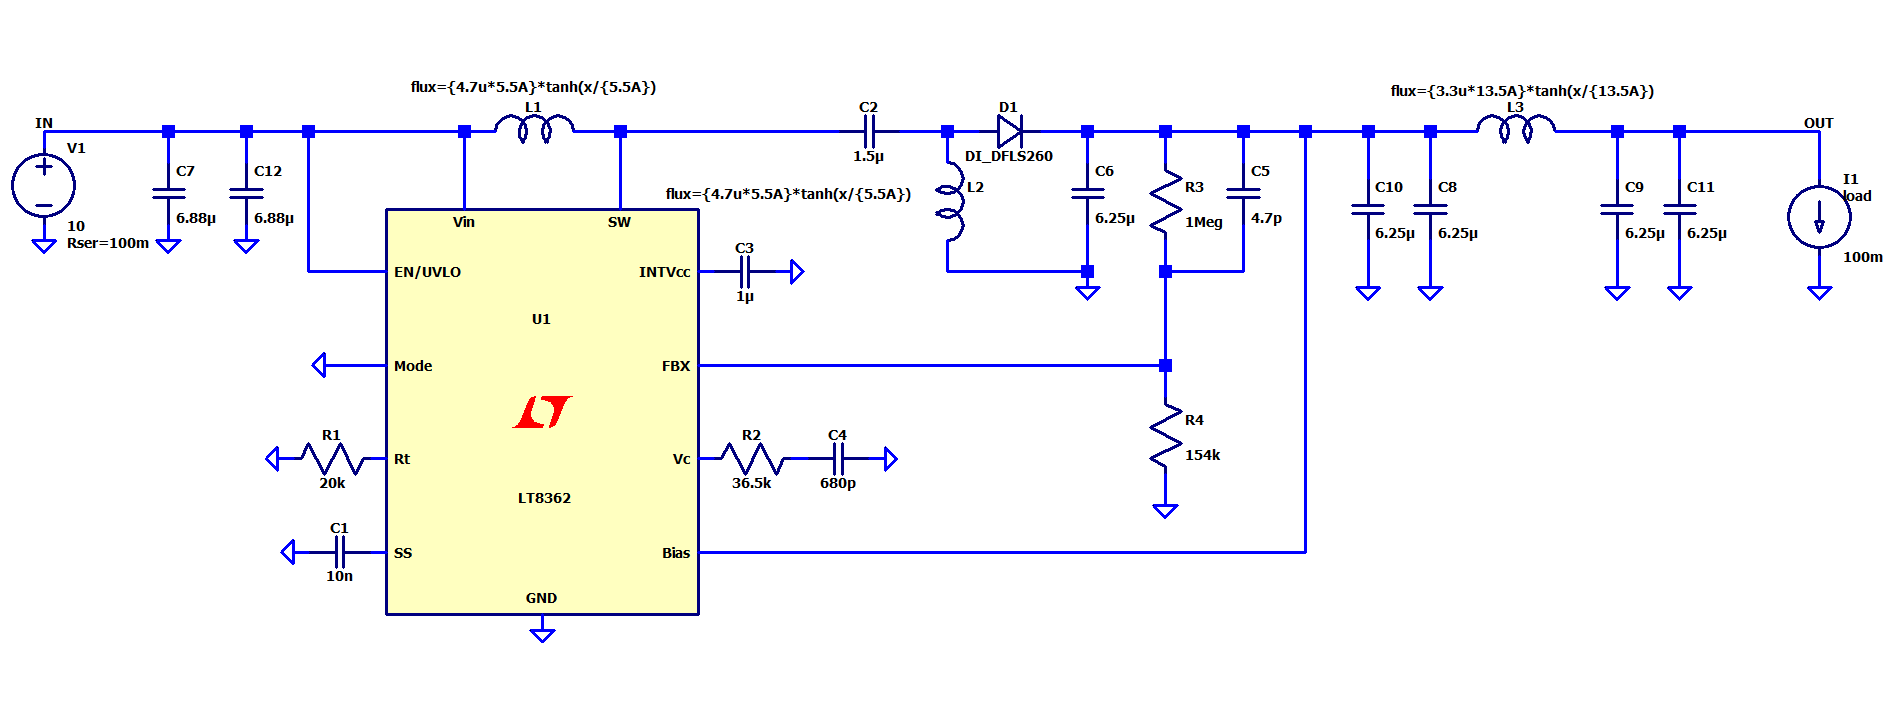
\includegraphics[width=\textwidth]{./figures/analog_2/schematic.png}
            \label{fig:subfig1}
        }
        \qquad
        \subfloat[Przebiegi czasowe prądu i napięcia na wyjściu układu]{
            \begin{tikzpicture}
                \pgfplotsset{
                    scale only axis,
                    scaled x ticks=base 10:3,
                    xmin=0, xmax=0.005
                }

                \begin{axis}[
                        grid=both,
                        axis y line*=left,
                        ymin=-1, ymax=14,
                        xlabel={Czas $t$ [s]},
                        ylabel={Napięcie wyjściowe $V_{\text{OUT}}$ [V]},
                    ]
                    \addplot[green, thick] table {./figures/analog_2/vout/segment_1.csv};\label{vout}
                    \addplot[green, thick] table {./figures/analog_2/vout/segment_2.csv};
                    \label{plot:vout}
                \end{axis}

                \begin{axis}[
                        axis y line*=right,
                        axis x line=none,
                        ymin=-0.02,
                        ymax=0.12,
                        ytick pos=right,
                        yticklabel pos=right,
                        ytick = {-0.02, 0, 0.02, 0.04, 0.06, 0.08, 0.1, 0.12},
                        yticklabels = {-20, 0, 20, 40, 60, 80, 100, 120},
                        ylabel={Prąd wyjściowy $I_{\text{OUT}}$ [mA]},
                        legend style={at={(0.95,0.05)},anchor=south east},
                    ]
                    \addlegendimage{/pgfplots/refstyle=vout}
                    \addlegendentry{$V_{OUT}$}
                    \addplot[red, thick] table {./figures/analog_2/iout/segment_1.csv};\label{iout}
                    \addplot[red, thick] table {./figures/analog_2/iout/segment_2.csv};

                    \addlegendimage{/pgfplots/refstyle=iout}
                    \addlegendentry{$I_{OUT}$}
                    \label{plot:current}
                \end{axis}
            \end{tikzpicture}

            \label{fig:subfig2}
        }
    \end{adjustbox}
\end{figure}

\subsection{Wybór elementów}
\subsubsection{Wybór LT8362}
Przetwornica obniżająca została wykonana w topologii SEPIC, ponieważ charakteryzują sie one mniejszymi tętnieniami napięcia wyjściowego niż przetwornice typu boost. Układ LT8362 został wybrany, ponieważ spełniał wymagania projektowe oraz był dostępny w dużych ilościach wśród dostawców. Dodatkowo, Analog Devices sugeruje go jako jeden z układów do wykorzystania przy nowych projektach.

\subsubsection{Dobór cewki}
Cewka została dobrana zgodnie ze wzorami dostępnym w nocie katalogowej, jednocześnie sugerując się przykładowym układem producenta. W układzie znalazła się cewka o wartości \SI{4.7}{\micro\henry}.

\subsubsection{Dobór kondensatorów}
Kondensatory zostały dobrane zgodnie z zaleceniami producenta układu, jednocześnie biorąc pod uwagę spadek pojemności. Wszystkie użyte kondensatory to kondensatory MLCC. Dokładna lista elementów znajduje się w pliku BOM.

\subsection{Filtr}
Na wyjściu układu umieszczony został filtr LP w topologii \Pi. Jego zadaniem jest usunięcie składowych wysoko-częstotliwościowych z napięcia wyjściowego, co przekłada się na zmniejszenie tętnień. W celu minimalizacji kosztów wykorzystana została taka sama cewka, jak w sekcji cyfrowej, wybrane zostały również wykorzystane wcześniej kondensatory \SI{10}{\micro\farad}. Pozwoliło to na uzyskanie częstotliwości granicznej: $$f_c = \frac{1}{2\pi \cdot \sqrt{L \cdot C}} = \frac{1}{2\pi \cdot \sqrt{\SI{3.3}{\micro\henry} \cdot \SI{10}{\micro\farad}}} = \SI{27.7}{\kilo\hertz}$$
W wyniku spadku pojemności kondensatorów rzeczywista częstotliwość graniczna wynosiłaby około $\SI{35}{\kilo\hertz}$. Jest to zmiana mająca pomijalny wpływ na działanie układu, jednakże w celu zbliżenia filtru do początkowo planowanego umieszczone zostały po dwa kondensatory na wejściu i wyjściu filtru. Dodanie kolejnego typu kondensatora byłoby zbędnym zwiększaniem kosztów produkcji układu.

\subsection{Wyniki symulacji}
\begin{table}[H]
    \centering
    \caption{Porównanie wyników symulacji w zależności od obciążenia}
    \label{tab:efficiency_ripple}
    \begin{tabular}{ccccc}
        \toprule
        \textbf{Prąd obciążenia [mA]} & \textbf{Sprawność [\%]} & $\mathbf{\Delta{V_{IN}} \ [mV]}$ & $\mathbf{\Delta{V_{OUT}} \ [mV]}$ & $\mathbf{V_{AVG} \ [V]}$ \\
        \midrule
        0.0                           & 0.00                    & 0.00                             & 0.76                              & -12.582                  \\
        10.0                          & 100.35                  & 11.97                            & 15.55                             & -12.005                  \\
        20.0                          & 97.88                   & 14.97                            & 19.46                             & -12.005                  \\
        30.0                          & 97.09                   & 16.89                            & 19.17                             & -12.005                  \\
        40.0                          & 96.49                   & 17.29                            & 14.32                             & -12.005                  \\
        50.0                          & 95.90                   & 14.91                            & 12.71                             & -12.005                  \\
        60.0                          & 96.04                   & 11.57                            & 10.68                             & -12.005                  \\
        70.0                          & 95.95                   & 1.75                             & 2.78                              & -12.005                  \\
        80.0                          & 95.95                   & 1.91                             & 2.75                              & -12.004                  \\
        90.0                          & 95.83                   & 2.19                             & 2.33                              & -12.004                  \\
        100.0                         & 95.73                   & 2.35                             & 2.93                              & -12.004                  \\
        \bottomrule
    \end{tabular}
\end{table}

\newpage
\section{Wnioski i podsumowanie}


\end{document}
